\documentclass{article} % For LaTeX2e
\usepackage{iclr2027_conference,times}

\usepackage[utf8]{inputenc}
\usepackage[T1]{fontenc}
\usepackage{hyperref}
\usepackage{url}
\usepackage{graphicx}
\usepackage{booktabs}
\usepackage{multirow}
\usepackage{amsmath,amssymb}
\usepackage{xcolor}
\usepackage{enumitem}
\usepackage{CJKutf8}
\usepackage[capitalise,nameinlink]{cleveref}
\crefname{figure}{Figure}{Figures}
\Crefname{figure}{Figure}{Figures}
\crefname{table}{Table}{Tables}
\Crefname{table}{Table}{Tables}

\newcommand{\bench}{\textsc{jy-crpg-bench}}
\newcommand{\game}[1]{\begin{CJK}{UTF8}{bsmi}#1\end{CJK}}
% A page holding only a float starts at the top, not centred.
\makeatletter\setlength{\@fptop}{0pt}\makeatother

% Anonymous ICLR submission: \iclrfinalcopy is off, so the style prints the
% review running head and the anonymous author block. For the camera-ready,
% restore \iclrfinalcopy and the author block.
% \iclrfinalcopy

\title{\raggedright\bench{}: A Long-Horizon Benchmark \\ for Frontier Models in an Open-World RPG}

\author{}

\begin{document}

\maketitle
% Figure 1 is placed in the introduction and belongs at the top of page 2;
% this keeps the title page free of top floats.
\suppressfloats[t]

%% Everything numeric in this paper is generated from the run data. Nothing is
%% typed. See figures/emit_numbers.py and check_consistency.py.
% generated by figures/numbers.py from catalog_snapshot.json and start.state
% regenerate before editing any number in the paper
% catalogue entries in the snapshot
\newcommand{\NsessionsTotal}{15}
% model sessions at the default budget that played
\newcommand{\Nsessions}{42}
% fewest sessions a model played
\newcommand{\LsessionsMin}{2}
% most sessions a model played
\newcommand{\LsessionsMax}{6}
% sessions at the default budget that played, the floor included
\newcommand{\NsessionsAll}{44}
% model sessions
\newcommand{\Nmodels}{42}
% random-baseline sessions
\newcommand{\NrandomRuns}{2}
% vendors in the field
\newcommand{\Nvendors}{5}
% distinct agent labels
\newcommand{\Nlabels}{13}
% distinct agent labels among the scored sessions
\newcommand{\NlabelsPlay}{12}
% distinct model labels among the scored sessions
\newcommand{\NmodelLabels}{12}
% distinct model names among the scored sessions
\newcommand{\NmodelsDistinct}{12}
% sessions that never sent a key
\newcommand{\Nnever}{3}
% sessions at another playtime
\newcommand{\NotherBudget}{0}
% service probes, excluded
\newcommand{\Nprobes}{0}
% default playtime, seconds
\newcommand{\Nbudget}{3600}
% default playtime, minutes
\newcommand{\NbudgetMin}{60}
% sessions on record created under a variant spelling of the model name
\newcommand{\Naliased}{10}
% the runs created under a name that was not the model, declared as listed
\newcommand{\aliaslist}{\texttt{GPT-5} as \texttt{gpt-5.6-sol} and \texttt{claude-fable-5.1-high} as \texttt{claude-fable-5.1} and \texttt{claude-fable5.1-high} as \texttt{claude-fable-5.1} and \texttt{claude-opus-5.5-high} as \texttt{claude-opus-5.5} and \texttt{claude-opus5-high} as \texttt{claude-opus-5} and \texttt{claude-sonnet-5-high} as \texttt{claude-sonnet-5} and \texttt{claude-sonnet5-high} as \texttt{claude-sonnet-5} and \texttt{glm-5.3-flash-high} as \texttt{glm-5.3-flash} and \texttt{opus5.5high} as \texttt{claude-opus-5.5}}
% reported sessions ended by the inactivity rule then in force
\newcommand{\Nidle}{11}
% reported sessions that played to their budget
\newcommand{\Ntime}{31}
% models with more than one session
\newcommand{\NrepeatModels}{2}
% sessions that give way to a longer one of the same model
\newcommand{\NrepeatSessions}{3}
% of those, sessions that never sent a key
\newcommand{\NrepeatNever}{3}
% model sessions at the default budget on record
\newcommand{\NsessionsRaw}{45}
% model sessions at the default budget that sent a key
\newcommand{\NsessionsPlayed}{42}
% most sessions any one model played
\newcommand{\NsessionsMaxPerModel}{6}
\newcommand{\EactsTotal}{15625}
\newcommand{\EactsModels}{15625}
\newcommand{\EactsRandom}{4236}
\newcommand{\EactsMedian}{199.5}
\newcommand{\EactsMin}{31}
\newcommand{\EactsMax}{1994}
% pooled actions per second
\newcommand{\Eaps}{0.118}
% screen reads by model sessions
\newcommand{\Ereads}{9057}
% model sessions in the cadence correlation
\newcommand{\NcadenceSessions}{42}
% of them with a count of screen reads
\newcommand{\NlookSessions}{24}
% median screen reads per action
\newcommand{\ClookMedian}{1.00}
% rank correlation of keys per action with milestones
\newcommand{\CrhoKeys}{-0.17}
% rank correlation of reads per action with milestones
\newcommand{\CrhoReads}{-0.28}
% key events submitted
\newcommand{\EkeysTotal}{49302}
% distinct keys submitted
\newcommand{\EkeysDistinct}{15}
% share on the four isometric axes
\newcommand{\EshareDiag}{0.922}
% share on the arrow keys
\newcommand{\EshareArrow}{0.014}
\newcommand{\EkeysEnter}{1915}
\newcommand{\EkeysSpace}{751}
% model sessions with at least thirty actions
\newcommand{\Nactive}{40}
\newcommand{\Qbest}{0.972}
\newcommand{\QbestLow}{0.947}
\newcommand{\QbestHigh}{0.986}
\newcommand{\QbestN}{290}
\newcommand{\QbestLabel}{gpt-6-astra}
\newcommand{\Qworst}{0.556}
\newcommand{\QworstLow}{0.509}
\newcommand{\QworstHigh}{0.602}
\newcommand{\QworstN}{439}
\newcommand{\QworstLabel}{gpt-5.6-sol}
\newcommand{\Qrandom}{0.422}
\newcommand{\QrandomLow}{0.408}
\newcommand{\QrandomHigh}{0.437}
\newcommand{\QrandomN}{4236}
\newcommand{\QrandomKeys}{13}
% budget the random floor ran at, minutes
\newcommand{\QrandomBudgetMin}{60}
% 1 when the floor ran at the default budget
\newcommand{\QrandomAtDefault}{1}
% active model sessions under the random floor
\newcommand{\NbelowFloor}{0}
\newcommand{\QunderVsRandom}{1.317}
% how many times below the random floor the lowest run sits
\newcommand{\QunderTimes}{0.8}
% the lowest active ratio as a multiple of the random floor
\newcommand{\QworstOverRandom}{1.3}
% median inter-action gap of the random baseline, seconds
\newcommand{\QrandomGap}{1.3}
% the seed of the random baseline
\newcommand{\QrandomSeed}{1996}
% its mean seconds between actions
\newcommand{\QrandomPace}{1.1}
% share of its draws that are a diagonal movement key, percent
\newcommand{\QrandomMoveShare}{67}
% share of its draws that are the confirm key, percent
\newcommand{\QrandomEnterShare}{12}
\newcommand{\QslowA}{gemini-3.7-flash}
\newcommand{\QslowB}{gemini-3.8-flash}
% the shorter of their median think times, seconds
\newcommand{\QslowGap}{20}
% the larger of their action counts
\newcommand{\QslowActs}{185}
% sessions whose character record was read
\newcommand{\Sread}{37}
\newcommand{\Sunread}{5}
% distinct levels among read records
\newcommand{\SlevelKinds}{1}
\newcommand{\Slevel}{1}
% experience accumulated by every run
\newcommand{\SexpSum}{0}
\newcommand{\Sskills}{1}
\newcommand{\SexpAny}{0}
\newcommand{\SlevelTwo}{0}
% sessions credited with the world map by the save the game wrote
\newcommand{\Smap}{32}
% sessions whose screen latched the world-map signature
\newcommand{\SmapScreen}{20}
% crossings carrying both a save and a fingerprint reading
\newcommand{\SmapBoth}{12}
% of those, crossings the fingerprint also shows
\newcommand{\SmapAgree}{11}
% crossings the save credits that the screen fingerprint missed
\newcommand{\SmapSaveOnly}{1}
% fingerprints with no save behind them, among sessions carrying both
\newcommand{\SmapScreenOnlyBoth}{0}
% screen latches with no save behind them
\newcommand{\SmapScreenOnly}{0}
% scored sessions that never reached the world map
\newcommand{\Sstayed}{10}
% crossings carrying the time of the first save
\newcommand{\SsaveN}{12}
% minutes into the session, median
\newcommand{\SsaveMedian}{21}
\newcommand{\SsaveFirst}{5}
\newcommand{\SsaveLast}{41}
% ratio of the steady-traversal run
\newcommand{\Qsteady}{0.972}
% its oscillation rate
\newcommand{\QsteadyOsc}{0.007}
% its action count
\newcommand{\QsteadyN}{290}
% its label
\newcommand{\QsteadyLabel}{gpt-6-astra}
% of those, corroborated by a black frame
\newcommand{\SmapFade}{20}
\newcommand{\SmapSolo}{0}
\newcommand{\SmapUnread}{16}
% minutes
\newcommand{\SexitMedian}{18.2}
\newcommand{\SexitFirst}{2.9}
\newcommand{\SexitLast}{36.6}
% median keypresses before a crossing
\newcommand{\SexitActs}{308}
% vendor families with a corroborated crossing
\newcommand{\SexitVendors}{5}
% sessions that picked something up
\newcommand{\Sitem}{19}
% sessions that never picked anything up
\newcommand{\SnoItem}{16}
\newcommand{\SitemKnown}{35}
% sessions holding the compass
\newcommand{\Scompass}{3}
% sessions whose save shows the scenes the hermit opens
\newcommand{\Sopened}{3}
\newcommand{\SopenedKnown}{28}
% the models holding the compass, by label
\newcommand{\ScompassLabel}{\texttt{claude-opus-5.5} and \texttt{gpt-6-astra}}
% minutes into the session when the compass holder's first save landed
\newcommand{\ScompassSaveMin}{5}
% actions the compass holder had taken at its crossing
\newcommand{\ScompassExitActs}{42}
\newcommand{\ScompassKnown}{21}
% sessions whose save the game wrote
\newcommand{\Ssaved}{23}
% sessions with a companion
\newcommand{\Steam}{0}
\newcommand{\SteamKnown}{21}
% sessions holding a book
\newcommand{\Sbooks}{0}
\newcommand{\SbooksKnown}{23}
% sessions that completed
\newcommand{\Sdone}{0}
% sessions that reached the map without the chest
\newcommand{\SleftNoItem}{13}
% sessions that searched the chest without reaching the map
\newcommand{\SitemNoLeft}{2}
% sessions that did both
\newcommand{\Sboth}{17}
% rungs the random floor reached, over its sessions
\newcommand{\QrandomRungs}{1}
% rungs on the ladder
\newcommand{\Lrungs}{11}
% rungs of the opening
\newcommand{\Lopening}{6}
% models on the ladder
\newcommand{\Lmodels}{12}
% models credited with rung 1
\newcommand{\Lmap}{12}
% models credited with rung 2
\newcommand{\Litem}{10}
% models credited with rung 3
\newcommand{\Lscene}{7}
% models credited with rung 4
\newcommand{\Lhermit}{5}
% models credited with rung 5
\newcommand{\Lcompass}{2}
% models credited with rung 6
\newcommand{\Lparty}{1}
% models credited with rung 7
\newcommand{\Lfight}{2}
% models credited with rung 8
\newcommand{\Lfought}{2}
% models credited with rung 9
\newcommand{\Lexp}{0}
% models credited with rung 10
\newcommand{\Llevel}{0}
% models credited with rung 11
\newcommand{\Lbook}{0}
% models that never picked anything up
\newcommand{\LnoItem}{2}
% models that never entered a scene beyond the home
\newcommand{\LnoScene}{5}
% the model with the most rungs
\newcommand{\LtopLabel}{\texttt{gpt-6-astra}}
% rungs it reached
\newcommand{\Ltop}{8}
% sessions it played
\newcommand{\LtopSessions}{4}
% the model whose crossings differ the most
\newcommand{\LspreadLabel}{\texttt{glm-5.3-flash}}
% factor between its slowest and fastest crossing
\newcommand{\LspreadRatio}{8}
% factor between the largest and smallest model mean
\newcommand{\LbetweenRatio}{6}
% fewest keypresses the top model took to the world map
\newcommand{\LtopCrossMin}{117}
% most keypresses it took
\newcommand{\LtopCrossMax}{134}
% the model session with the fewest keypresses to the world map
\newcommand{\LfewestKeysLabel}{\texttt{claude-opus-5.5}}
% fewest keypresses of any model session to the world map
\newcommand{\LfewestKeys}{110}
% in that many actions
\newcommand{\LfewestActs}{42}
% minute of that crossing
\newcommand{\LfewestMin}{3}
% model sessions credited with the world map
\newcommand{\LcrossSessions}{32}
% models that crossed in every session they played
\newcommand{\LcrossEvery}{7}
% other models that reached the hermit
\newcommand{\LhermitOthers}{4}
% sessions carrying both crossing counts, which agree on every one
\newcommand{\LcrossAgree}{20}
% the models that spoke with the hermit
\newcommand{\LhermitLabels}{\texttt{claude-opus-5.5}, \texttt{gemini-3.7-flash}, \texttt{gemini-3.8-flash}, \texttt{gpt-5.6-sol} and \texttt{gpt-6-astra}}
% random runs that wrote a save
\newcommand{\QrandomSaved}{0}
% sessions with a usage report
\newcommand{\Susage}{0}
% sessions that fetched the brief from the session
\newcommand{\Shelp}{5}
% scored sessions of the earlier twenty-minute field
\newcommand{\NoldSessions}{14}
\newcommand{\NoldBudgetMin}{20}
\newcommand{\NoldModels}{10}
\newcommand{\NoldLabels}{13}
\newcommand{\NoldVendors}{6}
% earlier sessions with a corroborated world-map crossing
\newcommand{\SoldMapFade}{3}
\newcommand{\SoldExpAny}{0}
% named scenes in the scene table
\newcommand{\Mscenes}{84}
% scenes open at the start
\newcommand{\MscenesOpenStart}{7}
% scenes open once the hermit has spoken
\newcommand{\MscenesOpenHermit}{80}
% scenes still closed after him
\newcommand{\MscenesClosedHermit}{4}
% character records addressed
\newcommand{\Mrecords}{320}
\newcommand{\MrecordBytes}{182}
% bytes of that block
\newcommand{\Mblock}{58240}
% records carrying a name
\newcommand{\Mnamed}{320}
% records exceeding hp/maxHp or mp/maxMp
\newcommand{\Moverflow}{2}
% key names the API accepts
\newcommand{\MkeyNames}{130}
% keys an action may carry
\newcommand{\MmaxKeys}{100}
% frames allowed for the game to react
\newcommand{\MsettleReact}{30}
% identical frames that count as settled
\newcommand{\MsettleStable}{9}
% frames after which the wait ends regardless
\newcommand{\MsettleMax}{120}
% distinct scancodes behind them
\newcommand{\MkeyCodes}{100}
% keypresses the slowest crossing took
\newcommand{\PexitActsMax}{1640}
\newcommand{\PexitActsMaxLabel}{\texttt{glm-5.3-flash}}
% minute of that crossing
\newcommand{\PexitMinMax}{37}
% sessions that never pressed enter or space
\newcommand{\PnoConfirm}{1}
\newcommand{\PorbitLabel}{\texttt{claude-fable-5.1}}
% minute it crossed
\newcommand{\PorbitExitMin}{13}
% actions it took on the world map afterwards
\newcommand{\PorbitActs}{1261}
% minutes it spent there
\newcommand{\PorbitMin}{44}
% distinct scenes the widest-ranging session entered
\newcommand{\PscenesMax}{4}
\newcommand{\PscenesMaxLabel}{\texttt{gpt-6-astra}}
% sessions that entered three or more distinct scenes
\newcommand{\PscenesThree}{3}
% confirm presses of its longest conversation
\newcommand{\PtalkHolderPresses}{42}
% minutes that conversation took
\newcommand{\PtalkHolderMin}{7}
% seconds a press
\newcommand{\PtalkHolderPace}{10}
% times it opened the item screen
\newcommand{\PholderMenuOpens}{9}
% arrow keys it pressed
\newcommand{\PholderArrows}{42}
% sessions that reached the hermit
\newcommand{\PhermitSessions}{9}
% earliest minute the top model reached the hermit
\newcommand{\PhermitTopFirst}{11}
% latest
\newcommand{\PhermitTopLast}{19}
% sessions of other models that reached him
\newcommand{\PhermitRestSessions}{5}
% earliest minute one of them did
\newcommand{\PhermitRestFirst}{31}
% latest
\newcommand{\PhermitRestLast}{53}
% earliest minute the top model read the compass
\newcommand{\PcompassTopFirst}{18}
% latest
\newcommand{\PcompassTopLast}{29}
% sessions that entered a fight
\newcommand{\PfightSessions}{3}
\newcommand{\LsecondLabel}{\texttt{claude-opus-5.5}}
% milestones the second model reached
\newcommand{\Lsecond}{7}
% its sessions
\newcommand{\LsecondSessions}{2}
% minute it entered the inn
\newcommand{\PsecondInnMin}{13}
% minute the compass entered its bag
\newcommand{\PsecondTakeMin}{33}
% minute it reached the hermit
\newcommand{\PsecondHermitMin}{31}
% minute its fight began
\newcommand{\PsecondBattleMin}{43}
% minute it read the compass
\newcommand{\PsecondCompassMin}{34}
% minute of its defeat banner
\newcommand{\PsecondDefeatMin}{47}
% minute the lost fight began
\newcommand{\PlostFightMin}{27}
% minute of the defeat banner
\newcommand{\PdefeatMin}{28}
% minute the compass was next read after the defeat
\newcommand{\PcompassAgainMin}{34}
% minute the standing fight began
\newcommand{\PbattleMin}{40}
% minute of that session's last key
\newcommand{\PbattleLastMin}{42}
% minute the companion's prompt first appeared
\newcommand{\PpromptMin}{52}
% minute it was answered yes
\newcommand{\PrecruitMin}{52}
% match threshold of the replay scan
\newcommand{\ReplayThreshold}{0.9}
% seconds of play a panel must stay above the threshold
\newcommand{\ReplayHold}{0.8}
% highest score of any frame without the event
\newcommand{\ReplayMissMax}{0.71}
% first panel readings checked by eye
\newcommand{\NpanelAudited}{20}
% sessions with both a bag reading and the message scan, which agree
\newcommand{\PobtainedAgree}{36}
% sessions whose item milestone is read from the message alone
\newcommand{\PobtainedRead}{8}
% lowest best score of a session with the event
\newcommand{\ReplayHitMin}{0.90}
% sessions with both a bag reading and a replay
\newcommand{\PcompassBoth}{21}
% of them whose bag holds the compass, all with the coordinate line on the replay
\newcommand{\PcompassBag}{3}
% sessions with a preserved save and a replay
\newcommand{\PhermitBoth}{30}
% of them whose save shows the scenes the hermit opens, all with his portrait on the replay
\newcommand{\PhermitOpened}{3}
% the model left out of the field
\newcommand{\LexcludedLabel}{\texttt{gemini-3.6-flash}}
% its sessions at the default budget in the catalogue
\newcommand{\NexcludedSessions}{2}
% sessions ended by the ten-minute idle rule the field ran with
\newcommand{\NidleSessions}{11}
% the days the field ran, UTC
\newcommand{\FieldDates}{10 to 12 September 2026}
\newcommand{\PtalkSlowLabel}{\texttt{gemini-3.8-flash}}
% confirm presses of the slowest conversation with the hermit
\newcommand{\PtalkSlowPresses}{40}
% minutes it took
\newcommand{\PtalkSlowMin}{15}
% seconds a press
\newcommand{\PtalkSlowPace}{23}
% minute it ended
\newcommand{\PtalkSlowEndMin}{54}
% minutes of budget left then
\newcommand{\PtalkSlowLeftMin}{6}
\newcommand{\PtalkFastLabel}{\texttt{gemini-3.7-flash}}
% confirm presses of the fastest conversation
\newcommand{\PtalkFastPresses}{60}
% minutes it took
\newcommand{\PtalkFastMin}{1}
% minute it began
\newcommand{\PtalkFastStartMin}{37}
% keys in the longest single action
\newcommand{\PbatchMaxKeys}{100}
\newcommand{\PbatchLabel}{\texttt{gpt-5.6-terra}}
% its keys per action
\newcommand{\PbatchKeysPerAction}{22}
% its actions of fifty keys or more
\newcommand{\PbatchBig}{32}
% attempts at the four-hour budget on record
\newcommand{\NlongAttempts}{48}
% four-hour sessions that count
\newcommand{\NlongSessions}{10}
% models with a four-hour session that counts
\newcommand{\NlongModels}{9}
% attempts that do not count
\newcommand{\NlongWithheld}{38}
% models with a four-hour attempt and no session that counts
\newcommand{\NlongPendingModels}{6}
% of them evaluated at the hour
\newcommand{\NlongFieldModels}{6}
\newcommand{\NlongFieldSessions}{7}
% requested wall-clock budget
\newcommand{\NlongBudgetMin}{240}
% the last key must fall within this many final minutes
\newcommand{\NlongWindowMin}{15}
\newcommand{\NlongMinLastMin}{225}
\newcommand{\NlongAliased}{8}
% attempts declared under names that identify no model of the paper
\newcommand{\NlongExcluded}{2}
% attempts of one or two actions
\newcommand{\NlongStartup}{3}
% attempts with no action
\newcommand{\NlongZero}{5}
% attempts whose harness read earlier sessions
\newcommand{\NlongProtocol}{1}
% attempts whose last key came before the final minutes
\newcommand{\NlongEarly}{27}
% the model whose attempt read the timelines of earlier sessions
\newcommand{\LlongHackLabel}{\texttt{gemini-3.8-flash}}
% models with a four-hour attempt and no session that counts
\newcommand{\LlongPendingLabels}{\texttt{deepseek-v4-flash}, \texttt{gemini-3.8-flash}, \texttt{gpt-5.6-terra}, \texttt{gpt-6-astra}, \texttt{grok-4.7} and \texttt{kimi-k3}}
% among the four-hour sessions that count
\newcommand{\NlongMap}{9}
% among the four-hour sessions that count
\newcommand{\NlongItem}{7}
% among the four-hour sessions that count
\newcommand{\NlongScene}{5}
% among the four-hour sessions that count
\newcommand{\NlongHermit}{1}
% among the four-hour sessions that count
\newcommand{\NlongCompass}{1}
% among the four-hour sessions that count
\newcommand{\NlongCompanion}{0}
% among the four-hour sessions that count
\newcommand{\NlongFight}{1}
% among the four-hour sessions that count
\newcommand{\NlongExp}{0}
% among the four-hour sessions that count
\newcommand{\NlongBook}{0}
% earliest last key, minutes
\newcommand{\LlongLastMin}{229.3}
% latest last key, minutes
\newcommand{\LlongLastMax}{239.8}
% earliest crossing, minutes
\newcommand{\LlongCrossFirst}{2.9}
% latest crossing, minutes
\newcommand{\LlongCrossLast}{52.4}
\newcommand{\NlongCrossLate}{0}
% the model of the four-hour session beyond the opening
\newcommand{\LlongBeyondLabel}{\texttt{claude-opus-5.5}}
% minute of its last key
\newcommand{\PlongBeyondLastMin}{229}
\newcommand{\PlongBeyondHermitMin}{31}
\newcommand{\PlongBeyondCompassMin}{34}
\newcommand{\PlongBeyondBattleMin}{43}
\newcommand{\PlongBeyondDefeatMin}{47}
\newcommand{\LfirstHourLabel}{\texttt{claude-opus-5.5}}
% its four-hour sessions read over their first hour
\newcommand{\NfirstHourSessions}{2}
% the days the four-hour sessions that count ran, UTC
\newcommand{\LongDates}{16 to 22 September 2026}
% the least match of the opening room that admits a capture
\newcommand{\HumanRoomGate}{0.90}
% published videos of human players the paper reads
\newcommand{\NhumanVideos}{7}
\newcommand{\NhumanSpeedruns}{4}
\newcommand{\NhumanPlaythroughs}{3}
% speedrun: earliest minute of map
\newcommand{\LhumanSpeedMapFirst}{0.1}
% speedrun: latest minute of map
\newcommand{\LhumanSpeedMapLast}{0.5}
% speedrun: earliest minute of hermit
\newcommand{\LhumanSpeedHermitFirst}{0}
% speedrun: latest minute of hermit
\newcommand{\LhumanSpeedHermitLast}{2}
% speedrun: earliest minute of fight
\newcommand{\LhumanSpeedFightFirst}{1}
% speedrun: latest minute of fight
\newcommand{\LhumanSpeedFightLast}{3}
% speedrun: earliest minute of book
\newcommand{\LhumanSpeedBookFirst}{26}
% speedrun: latest minute of book
\newcommand{\LhumanSpeedBookLast}{72}
\newcommand{\LhumanSpeedStepsMin}{32}
\newcommand{\LhumanSpeedStepsMax}{107}
% speedrun videos in which the compass is taken
\newcommand{\NhumanSpeedCompass}{2}
% speedrun videos that reach a book
\newcommand{\NhumanSpeedBook}{4}
% speedrun videos that finish the game
\newcommand{\NhumanSpeedComplete}{4}
\newcommand{\LhumanSpeedCompletionMin}{60}
\newcommand{\LhumanSpeedCompletionMax}{126}
% playthrough: earliest minute of map
\newcommand{\LhumanPlayMapFirst}{0.4}
% playthrough: latest minute of map
\newcommand{\LhumanPlayMapLast}{1.6}
% playthrough: earliest minute of hermit
\newcommand{\LhumanPlayHermitFirst}{1}
% playthrough: latest minute of hermit
\newcommand{\LhumanPlayHermitLast}{3}
% playthrough: earliest minute of fight
\newcommand{\LhumanPlayFightFirst}{7}
% playthrough: latest minute of fight
\newcommand{\LhumanPlayFightLast}{13}
% playthrough: earliest minute of book
\newcommand{\LhumanPlayBookFirst}{58}
% playthrough: latest minute of book
\newcommand{\LhumanPlayBookLast}{105}
\newcommand{\LhumanPlayStepsMin}{100}
\newcommand{\LhumanPlayStepsMax}{121}
% playthrough videos in which the compass is taken
\newcommand{\NhumanPlayCompass}{3}
% playthrough videos that reach a book
\newcommand{\NhumanPlayBook}{3}
% playthrough videos that finish the game
\newcommand{\NhumanPlayComplete}{1}
\newcommand{\LhumanPlayCompletionMin}{273}
\newcommand{\LhumanPlayCompletionMax}{273}
% --- derived strings used by the results table -------------------------
% each row: agent & second & first & keys & screen-changing decisions/n & ratio\ci{n} & in-going & map & end
% rows below are sorted by vendor then actions
% claude-fable-5.1           n=1592 k=1321 ratio=0.830[0.811,0.847] map=True level=1 exp=0 ttfa=20.43 reason=time
% claude-opus-5.5            n=1094 k=   0 ratio=0.000[0.000,0.003] map=True level=1 exp=0 ttfa=0.0 reason=time
% claude-opus-5.5            n= 825 k=   0 ratio=0.000[0.000,0.005] map=True level=1 exp=0 ttfa=0.0 reason=time
% claude-sonnet-5            n= 377 k= 346 ratio=0.918[0.886,0.941] map=True level=1 exp=0 ttfa=17.04 reason=time
% claude-sonnet-5            n= 361 k= 289 ratio=0.801[0.756,0.839] map=True level=1 exp=0 ttfa=12.97 reason=time
% claude-opus-5              n= 341 k= 268 ratio=0.786[0.739,0.826] map=True level=1 exp=0 ttfa=15.83 reason=time
% claude-opus-5              n= 265 k= 218 ratio=0.823[0.772,0.864] map=True level=1 exp=0 ttfa=31.5 reason=time
% claude-fable-5.1           n= 155 k= 122 ratio=0.787[0.716,0.844] map=True level=1 exp=0 ttfa=28.69 reason=idle
% gemini-3.7-flash           n= 344 k= 303 ratio=0.881[0.842,0.911] map=None level=1 exp=0 ttfa=None reason=time
% gemini-3.8-flash           n= 199 k= 168 ratio=0.844[0.787,0.888] map=True level=1 exp=0 ttfa=15.3 reason=time
% gemini-3.8-flash           n= 185 k= 154 ratio=0.832[0.772,0.879] map=True level=1 exp=0 ttfa=94.69 reason=time
% gemini-3.7-flash           n= 180 k= 155 ratio=0.861[0.803,0.904] map=True level=1 exp=0 ttfa=16.24 reason=time
% gemini-3.8-flash           n= 163 k= 130 ratio=0.798[0.729,0.852] map=None level=1 exp=0 ttfa=None reason=time
% gemini-3.7-flash           n= 160 k= 116 ratio=0.725[0.651,0.788] map=None level=1 exp=0 ttfa=None reason=time
% gemini-3.7-flash           n= 102 k=  90 ratio=0.882[0.806,0.931] map=True level=1 exp=0 ttfa=26.41 reason=time
% gemini-3.8-flash           n=  31 k=  29 ratio=0.935[0.793,0.982] map=None level=None exp=None ttfa=None reason=idle
% glm-5.3-flash              n=1994 k=1872 ratio=0.939[0.927,0.949] map=True level=1 exp=0 ttfa=47.66 reason=time
% glm-5.3-flash              n= 920 k= 797 ratio=0.866[0.843,0.887] map=False level=1 exp=0 ttfa=20.46 reason=time
% glm-5.3-flash              n= 215 k= 184 ratio=0.856[0.803,0.897] map=True level=1 exp=0 ttfa=14.65 reason=time
% glm-5.3-flash              n= 200 k= 147 ratio=0.735[0.670,0.791] map=None level=None exp=None ttfa=None reason=time
% glm-5.3-flash              n= 167 k= 135 ratio=0.808[0.742,0.861] map=None level=1 exp=0 ttfa=None reason=time
% gpt-5.6-sol                n=1559 k=1077 ratio=0.691[0.667,0.713] map=True level=1 exp=0 ttfa=13.45 reason=time
% gpt-5.6-sol                n= 439 k= 244 ratio=0.556[0.509,0.602] map=None level=None exp=None ttfa=None reason=time
% gpt-6-astra                n= 290 k= 282 ratio=0.972[0.947,0.986] map=True level=1 exp=0 ttfa=19.31 reason=time
% gpt-6-astra                n= 259 k= 243 ratio=0.938[0.902,0.962] map=None level=1 exp=0 ttfa=None reason=idle
% gpt-6-astra                n= 250 k= 232 ratio=0.928[0.889,0.954] map=True level=1 exp=0 ttfa=26.78 reason=time
% gpt-5.6-sol                n= 225 k= 198 ratio=0.880[0.831,0.916] map=True level=1 exp=0 ttfa=23.29 reason=time
% gpt-5.6-terra              n= 208 k= 154 ratio=0.740[0.677,0.795] map=None level=1 exp=0 ttfa=None reason=idle
% gpt-5.6-sol                n= 183 k= 131 ratio=0.716[0.647,0.776] map=None level=1 exp=0 ttfa=None reason=idle
% gpt-5.6-luna               n= 180 k= 133 ratio=0.739[0.670,0.798] map=False level=1 exp=0 ttfa=11.62 reason=time
% gpt-5.6-luna               n= 175 k= 140 ratio=0.800[0.735,0.853] map=True level=1 exp=0 ttfa=9.22 reason=idle
% gpt-5.6-terra              n= 163 k= 125 ratio=0.767[0.696,0.825] map=False level=1 exp=0 ttfa=11.94 reason=time
% gpt-5.6-luna               n= 155 k= 135 ratio=0.871[0.809,0.915] map=None level=1 exp=0 ttfa=None reason=time
% gpt-5.6-terra              n= 135 k=  94 ratio=0.696[0.614,0.768] map=None level=None exp=None ttfa=None reason=time
% gpt-5.6-luna               n= 133 k=  95 ratio=0.714[0.632,0.784] map=None level=1 exp=0 ttfa=None reason=idle
% gpt-6-astra                n= 128 k= 124 ratio=0.969[0.922,0.988] map=None level=1 exp=0 ttfa=None reason=time
% gpt-5.6-terra              n= 118 k=  82 ratio=0.695[0.607,0.771] map=False level=1 exp=0 ttfa=9.98 reason=idle
% gpt-5.6-luna               n=  94 k=  62 ratio=0.660[0.559,0.747] map=False level=1 exp=0 ttfa=12.83 reason=idle
% gpt-5.6-terra              n=  70 k=  42 ratio=0.600[0.483,0.707] map=False level=1 exp=0 ttfa=10.3 reason=idle
% gpt-5.6-terra              n=  48 k=  37 ratio=0.771[0.635,0.867] map=None level=None exp=None ttfa=None reason=idle
% grok-4.6                   n= 597 k= 422 ratio=0.707[0.669,0.742] map=None level=1 exp=0 ttfa=None reason=time
% grok-4.6                   n= 346 k= 277 ratio=0.801[0.755,0.839] map=True level=1 exp=0 ttfa=16.52 reason=time
% --- repetition of a label appears in the catalogue ----------------------------
% repeated claude-sonnet-5: [0.8005540166204986, 0.9177718832891246] spread=0.117
% repeated claude-fable-5.1: [0.8297738693467337, 0.7870967741935484] spread=0.043
% repeated claude-opus-5: [0.7859237536656891, 0.8226415094339623] spread=0.037
% repeated glm-5.3-flash: [0.9388164493480441, 0.866304347826087, 0.735, 0.8083832335329342, 0.8558139534883721] spread=0.204
% repeated gpt-6-astra: [0.928, 0.9382239382239382, 0.96875, 0.9724137931034482] spread=0.044
% repeated gpt-5.6-terra: [0.7668711656441718, 0.7403846153846154, 0.7708333333333334, 0.6962962962962963, 0.6, 0.6949152542372882] spread=0.171
% repeated gpt-5.6-sol: [0.88, 0.7158469945355191, 0.5558086560364465, 0.6908274534958306] spread=0.324
% repeated gpt-5.6-luna: [0.7388888888888889, 0.7142857142857143, 0.8709677419354839, 0.8, 0.6595744680851063] spread=0.211
% repeated grok-4.6: [0.8005780346820809, 0.7068676716917923] spread=0.094
% repeated gemini-3.7-flash: [0.8823529411764706, 0.8808139534883721, 0.725, 0.8611111111111112] spread=0.157
% repeated gemini-3.8-flash: [0.8324324324324325, 0.9354838709677419, 0.7975460122699386, 0.8442211055276382] spread=0.138
% repeated claude-opus-5.5: [0.0, 0.0] spread=0.000

% generated by figures/emit_books.py from server/save_state.py
\newcommand{\BookFirst}{144}
\newcommand{\BookLast}{157}
\newcommand{\BookCount}{14}
\newcommand{\booktable}{The Young Flying Fox & \game{飛狐外傳} \\ Fox Volant of the Snowy Mountain & \game{雪山飛狐} \\ A Deadly Secret & \game{連城訣} \\ Demi-Gods and Semi-Devils & \game{天龍八部} \\ The Legend of the Condor Heroes & \game{射鵰英雄傳} \\ White Horse Neighs in the Western Wind & \game{白馬嘯西風} \\ The Deer and the Cauldron & \game{鹿鼎記} \\ The Smiling, Proud Wanderer & \game{笑傲江湖} \\ The Book and the Sword & \game{書劍恩仇錄} \\ The Return of the Condor Heroes & \game{神鵰俠侶} \\ Ode to Gallantry & \game{俠客行} \\ The Heaven Sword and Dragon Saber & \game{倚天屠龍記} \\ Sword Stained with Royal Blood & \game{碧血劍} \\ Blade-dance of the Two Lovers & \game{鴛鴦刀} \\}
\newcommand{\CompassId}{182}
\newcommand{\DefaultBudgetSec}{14400}
\newcommand{\DefaultBudgetMin}{240}
\newcommand{\DefaultReplaySpeed}{8}


\begin{abstract}
A long-horizon task requires a model to perceive its environment, decide for
itself what is worth doing, and hold one plan across hours of dependent
decisions. We present \bench{}, which places a frontier model inside Heroes of Jin Yong, a 1996 open-world role-playing game run under DOS emulation. Its ending requires the fourteen books of the Jin Yong novels and takes a first-time human player tens of hours. The game requires reading $320\times200$ isometric pixel art and 16-pixel Traditional Chinese, knowledge of the novels its world is built from, and a keyboard as the only actuator. It has no quest log, marker or score, so the model must maintain its own map and goals, and it must win turn-based fights against the game AI. Progress is scored by milestones of the game itself and, once a model finishes, by completion time. Under a
\NbudgetMin{}-minute budget, in which a human speedrun finishes the game, one of \NmodelsDistinct{} frontier models plays
past the opening of the game, and none gains experience or holds a book. Four-hour sessions of \NlongModels{} models that play to their budget stay inside the opening.
\end{abstract}

\section{Introduction}
\label{sec:intro}

Frontier models solve competition mathematics and write working compilers,
yet the tasks they complete reliably are still measured in hours of human
work \citep{kwa2025horizon}. A long horizon is a property of the task, the
number of dependent steps its completion requires \citep{chen2026horizongap},
and several of the benchmarks that measure it are text environments, business
simulations \citep{backlund2025vending,fan2026ecommerce} or interactive
fiction \citep{phan2025textquests}. A game adds a requirement they leave
out: the model has to recover its own state from raw perception, because
nothing in the environment reports it. The game benchmarks that keep perception each relax another part of the problem: BALROG adds a text rendering of the state \citep{paglieri2025balrog}, ARC-AGI-3 removes language \citep{arc2026arcagi3}, and MineExplorer hands the model its objectives \citep{ju2026mineexplorer}. None combines raw pixels, a non-English script and self-directed play, as \cref{tab:related} shows.

\begin{figure}[!htb]
\centering
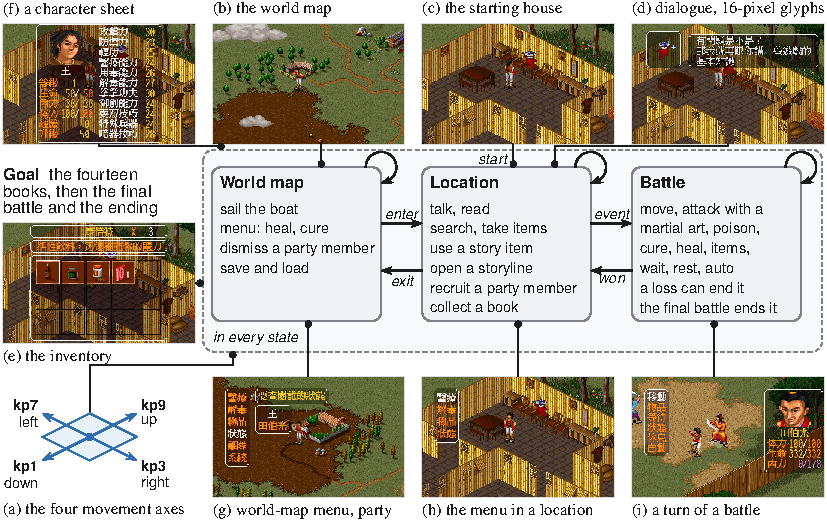
\includegraphics[width=\linewidth]{figures/env.pdf}
\caption{The environment as the model receives it, upscaled three times without interpolation.}
\label{fig:env}
\end{figure}

We present \bench{}, built on Heroes of Jin Yong (\game{金庸群俠傳}), a 1996 Chinese role-playing game that we run as its original DOS binary under emulation. Its ending requires recovering the fourteen books of the Jin Yong novels from an open world, a task that takes a first-time human player tens of hours, and \cref{fig:env} shows its world. We chose the game because it tests five capabilities of a frontier model at once.
\begin{enumerate}[leftmargin=*,topsep=2pt,itemsep=1pt,parsep=0pt]
\item The model must read the screen. The frame is $320\times200$ pixel art in a $45^\circ$ isometric projection, and every objective, prompt and statistic on it is Traditional Chinese in 16-pixel glyphs, a script that multimodal evaluation has largely neglected \citep{tam2025vistw}. No text is supplied to the model.
\item The model must bring knowledge the game never states. The world is assembled from the fourteen novels, so who a character is, which faction to join and which storyline leads to a book are known to a reader of the novels and written nowhere on screen.
\item The model must set its own goals. The game keeps no quest log, draws no marker and reports no score, so the model maintains its own map and plan and decides for itself what is worth doing. ARC-AGI-3 places the same goal-setting requirement at the centre of agentic intelligence \citep{arc2026arcagi3}.
\item The model must act through a keyboard alone, exposed through an API that it calls as a tool. Movement runs along four diagonals, no key moves straight up the screen, and every system of the game is a menu.
\item The model must win fights. Fights are turn-based on a grid against the AI of the game, with position, range and inner force to manage, and a party at level one can lose them.
\end{enumerate}
Together these form one long-horizon task, a persistent world with sparse and delayed reward over thousands of dependent steps. This is the setting of reinforcement learning, and here a frontier model plays it in context, with no training on the game. Two further properties make the game a usable benchmark. It is menu-driven, so a model that deliberates between actions is not penalised as in a real-time game \citep[cf.][]{zhang2025videogamebench}, and its progression state is measurable per character, so progress is scored against events of the game itself.

The next section reviews these benchmarks, \cref{sec:bench} details the
environment, the interface, the session protocol and the measurement, and \cref{sec:results} reports which milestones the models reach and how they play.

\begin{table}[!htb]
\centering
\caption{Interactive agent benchmarks. Observation is what the model receives before any upscaling, a self-directed environment supplies no task list, score or objective marker during play, and the last column is the record that verifies progress.}
\label{tab:related}
\footnotesize
\setlength{\tabcolsep}{2pt}
\begin{tabular}{@{}llllcl@{}}
\toprule
Benchmark & Environment & Observation & Language & Self-directed & Progress from \\
\midrule
\textbf{\bench{}} & one 1996 CRPG & 320$\times$200 px & Trad.\ Chinese & yes & memory, save, replay \\
\midrule
BALROG & 6 research games & text, render & English & no & env.\ reward \\
TextQuests & interactive fiction & text & English & yes & game state \\
ARC-AGI-3 & abstract puzzles & 64$\times$64 grid & none & yes & env.\ score \\
VideoGameBench & 1990s action games & native px & English & no & checkpoint images \\
GameWorld & 34 browser games & browser & English & no & game state \\
MineExplorer & Minecraft & 3D render & English & no & milestone rules \\
\bottomrule
\end{tabular}
\end{table}

\section{Related Work}
\label{sec:related}

\subsection{Game Environments as Agent Benchmarks}

Games have been the standard setting for sequential decision-making since the
Arcade Learning Environment \citep{bellemare2013arcade}, and language and
vision-language agents have produced a second generation of game benchmarks.
BALROG aggregates six reinforcement-learning environments under one protocol
and reports a persistent gap between what a model knows about a game and what
it does inside one \citep{paglieri2025balrog}. lmgame-Bench isolates how much
of a game result belongs to the harness \citep{hu2026lmgame}, and Orak spans
twelve popular titles with configurable agentic modules \citep{park2026orak}.
VideoGameBench is the nearest benchmark to ours, running real 1990s games from raw pixels under a no-scaffold rule \citep{zhang2025videogamebench}.
GameWorld
standardises the action interface across 34 browser games and pairs every
task with a state-verifiable metric \citep{ouyang2026gameworld}. MineExplorer
evaluates open-world exploration in Minecraft and finds that models handle
single-hop tasks but degrade once hidden prerequisites must be coordinated
over a longer trajectory \citep{ju2026mineexplorer}.

The nearest precedents in horizon are the public Pok\'emon runs. Claude 3.7 Sonnet reached three
gym badges from screen pixels with a memory scaffold, where an earlier
model had not left the first house \citep{anthropic2025pokemon}. Gemini 2.5
Pro finished Pok\'emon Blue in 813 hours with a harness that translated the
RAM of the game into text, and an ablation without vision performed about as
well \citep{comanici2025gemini}. The PokeAgent Challenge turned the setting
into a speedrunning track scored by completion time over milestones
\citep{karten2026pokeagent}. PokeGym builds a long-horizon benchmark on the
open-world game Pok\'emon Legends: Z-A with no access to game state
\citep{zhang2026pokegym}, and StarBench one on the turn-based Honkai: Star
Rail \citep{zhang2025starbench}. Crafter established the single-environment,
achievement-based design we follow \citep{hafner2021benchmarking}, and
NetHack remains the deepest environment in use for learned agents, with runs of tens of thousands of turns \citep{kuttler2020nethack}. Cradle and Voyager drive games through a foundation model with a skill library or a code API \citep{tan2024cradle,wang2023voyager}.

\subsection{Long-Horizon Evaluation and Its Measurement}

Vending-Bench established long-term coherence as the property that separates
long-horizon tasks from long chains of short ones
\citep{backlund2025vending}, and E-Commerce Bench extends the setting
to a year of deterministic business operation
\citep{fan2026ecommerce}. Both keep perception out of the loop. TextQuests
shares our self-directed, long-horizon framing while removing vision \citep{phan2025textquests}, and TextAtari stretches horizons to $10^5$ steps over
text renderings \citep{li2025textatari}. ARC-AGI-3 isolates adaptation to
novel tasks by excluding language and external knowledge
\citep{arc2026arcagi3}, and AutumnBench probes
world-model quality through environment-level queries
\citep{warrier2025benchmarking}. UltraHorizon makes exploration under hidden
rules the task itself \citep{luo2025ultrahorizon}, and \citet{kapoor2026openworld}
observe that benchmark design has favoured tasks that are precisely
specified, automatically graded and short, and call for open-world
evaluation. Navigation is a documented weakness even without perception: one-shot maze navigation fails by ten cells a side for every model tested \citep{jiang2026lostaggregation}, and from coordinates alone the failures are attributed to looping \citep{einarsson2025mazeeval}.

Long horizons also complicate measurement. The ABC checklist
catalogues task-validity and outcome-validity failures across agentic
benchmarks \citep{zhu2025establishing}. An audit of agent traces finds
reward hacking in a majority of them on two suites \citep{shao2026validity},
and a survey of the horizon gap finds that the field answers uninformative
outcome signals by building denser step-level ones
\citep{chen2026horizongap}. State-based verification has precedent outside
games, where $\tau$-bench compares the final database state with an
annotated goal \citep{yao2024taubench}.

\section{\bench{}}
\label{sec:bench}

\subsection{Environment}
\label{sec:env}

Heroes of Jin Yong, published by Heluo Studio (\game{河洛工作室}) in 1996, is an open world of two tiers: many local scenes such as buildings, sects and caves attached to one world map of $480\times480$ tiles \citep{scarsty2026kyscpp}. Each of \Mrecords{} named characters carries a record of level, experience, health, stamina, skills, items, reputation and aptitude, and every scene carries an entry condition. Of the \Mscenes{} scenes, \MscenesOpenStart{} are open at the start: the home, five inns (\game{客棧}) and the house of the hermit (\game{南賢}). The conversation with the hermit opens all but \MscenesClosedHermit{} of the rest, and from there the order of play is left to the player. The only instruction the game gives comes from its fiction: enter the world of the Jin Yong novels, join its factions, learn its martial arts, and recover the fourteen books that end the game.

The game fixes the order of its opening and leaves the campaign open. It starts in a small compound with a searchable chest, one speaking character and one exit tile, and beyond the exit the path south across the world map leads to the hermit. \Cref{fig:route} in \cref{app:infra} shows the route. A cabinet beside him holds the compass (\game{羅盤}), the only source of coordinates the game offers, and his conversation opens the house of the first companion, who joins after a yes-or-no prompt at which the confirm key means no. The opening ends there and needs no fight. The campaign that follows runs through fights, the experience and levels that victories bring, and the chains of items, factions and fights that lead to the books. Fights are turn-based on the scene grid: each turn a character moves along the four axes and then strikes, uses an item, waits or rests, and skills draw on inner force (\game{內力}). The first scripted fight begins with the party drained of it, and a party that goes elsewhere first meets storylines whose fights it cannot survive at level one. Some of these fights end the game when lost, leaving only the load menu, and others let the story continue. With all fourteen books and enough reputation, the ending is a boss fight at a shrine on the far side of the world map \citep{bahamut2023walkthrough}.

The two phases test different capabilities. The opening is played by walking, reading and answering, and we give the model the route as far as the compass, so a stall there is a failure of perception or navigation. The campaign adds combat and the knowledge of the novels, since the game names its characters, factions and storylines and explains none of them. \Cref{app:licence} states the licences of the benchmark code, the emulator and the game.

\subsection{Observation and Action Space}
\label{sec:interface}

The model observes the raw framebuffer at $320\times200$ and acts by pressing
keys. A scored session serves the native frame without upscaling, annotation,
set-of-marks overlay or accessibility tree \citep[cf.][]{xie2024osworld}. The frame combines several documented weaknesses of vision-language models. Low resolution reduces their accuracy \citep{niu2025resolution}, and images far from the training distribution degrade recognition even of familiar categories \citep{lin2026oodbench}. Text rendered as pixels is understood less well than the same text supplied as
tokens \citep{liu2026vistabench}, and precise spatial reading fails once
primitives are small or adjacent
\citep{rahmanzadehgervi2024blind,wang2024spatialeval}. The action space is
the DOS keyboard, with \MkeyNames{} key names over
\MkeyCodes{} distinct keys, and \cref{fig:keymap} shows the few the game responds to. Movement runs along the four numpad diagonals, with the arrow
keys aliased onto the same axes, so a model that presses \texttt{up} expecting
to walk up the screen moves up and to the right.

The single action presses a key, or a list of up to \MmaxKeys{} keys in order, holding each for a requested number of emulated frames. It returns once the screen has settled, including after a scene change, so the frame the model receives is the one to act on. There is no call that advances the game without input. A scored session answers four of the calls in \cref{tab:api} and refuses the three that save, list and restore emulator snapshots, so a run cannot be rewound from outside the game. The save and load menu of the game stays available to the model, as it is to a human player, so a model that loses a fight can reload the last save the game wrote. \Cref{app:infra} states the settle rule in frames, and \cref{app:design} gives the reasons for the list action and for the other choices of the protocol.

\subsection{Harness and Session Protocol}
\label{sec:protocol}

The benchmark supplies the brief and the control surface, and the model plays through an agent harness. Every model in this paper ran inside pi\footnote{\url{https://github.com/badlogic/pi-mono}}, a minimal coding agent, installed without modification and set to its high thinking level. Its four tools read, write and edit files and run a shell, from which the model drives the control surface with HTTP calls. The brief is the whole instruction the model receives. It covers the session call, the calls that constitute play, the opening route as far as the compass, and a manual of the controls and systems of the game. It is published as \texttt{agents.md}, the project file pi reads at launch, in English and in Chinese, and both versions keep the on-screen Traditional Chinese terms verbatim. An action returns only its metadata unless the model asks for the frame in the same reply, so the model looks at the screen when it decides to. The benchmark adds no memory scaffold, no map, no pathfinder and no access to the state of the game. A model keeps any memory between actions in files it writes in that shell, and a scored session receives no field that reports its progress until the run ends, so a model cannot query its own score. The catalogue is served only to the leaderboard page, the run store refuses listing, and a container profile runs the harness without network access beyond its own session. The leaderboard therefore ranks models under one fixed harness, since harness choice changes game results \citep{hu2026lmgame,karten2026harness} and on long-horizon tasks the variance a harness induces can exceed the variance between models \citep{zhang2026harness}.

A session is created with a declared model name and a playtime of
\DefaultBudgetMin{} minutes by default and at most twenty-four hours, and its
clock starts at the first playable moment. The server keeps the wall clock of every decision call, so played time and think time are measured for any client. Each session is a separate emulator process with a private copy of the game, supplied by the host, with its save slots reset to a new game, so no run inherits the progress of another. A session ends when its budget lapses or the game is completed. When the budget lapses the session renders its recording to a time-compressed
video, computes its metrics, and appends itself to the public catalogue with the video and its keypress timeline. \Cref{fig:apparatus} shows the apparatus, and \cref{app:infra} lists the emulation and hosting parameters.

\begin{figure}[!htb]
\centering
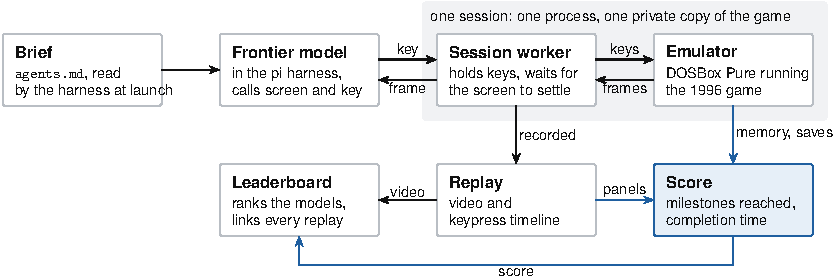
\includegraphics[width=\linewidth]{figures/architecture.pdf}
\caption{A frontier model in pi drives the control API of its own session. The recording feeds the public replay, and progress is read from the emulated machine, the save the game writes and the replay, none of which the control API exposes.}
\label{fig:apparatus}
\end{figure}

\subsection{Measuring Progress}
\label{sec:measure}

Progress is read from three records that the control surface never exposes: the memory of the emulated machine, the save the game writes, and the published replay. The game keeps its persistent state in one archive, with the world position, the party roster and the shared bag in front of the \Mrecords{} character records, and the bag is the working copy that changes the moment an item is taken. From the live machine the benchmark reads the item count, the compass and the books after every action, and the level and experience of every character. The party roster and the world position are read from the save the game writes. The game offers its save menu on the world map alone and draws it with six rows there and four in a scene, so every two minutes the benchmark presses one escape while the model is idle and saves when the menu has six rows. A successful save is therefore the evidence that the party has crossed onto the world map, and the first one times the crossing. The session is held while the attempt runs, so the model never sees the screen mid-save, and its few seconds of menu time are not charged to the run.

Six events leave no trace in either record, because the game keeps them only on screen. The model enters a scene from the world map, speaks with the hermit, opens the item screen with the compass in it, enters a fight, loses it, or answers the prompt of a companion who asks to join. Each draws fixed art at a fixed screen position, so these events are read from the published replay by matching every frame against that art. The readings do not alter the game: the benchmark serialises the machine and never loads state into it, and the only keys it presses on its own belong to the save attempt. A milestone, once observed, stays credited, so an item picked up and later used still counts. \Cref{app:measure} lists the record behind each milestone, the rules of the save attempt and the panel matching, and checks the readings against one another wherever two records exist.

The milestone scale has \Lrungs{} steps, following the achievements of Crafter \citep{hafner2021benchmarking}: six in the opening and five in the campaign. The opening milestones are the exit tile, the chest in the first room, a scene entered from the world map, the conversation with the hermit, the compass in his cabinet, and the companion who joins through dialogue. The campaign milestones are a fight entered, a fight fought to its end, experience gained, the second level, and the first of the fourteen books. The milestones are listed in the order of the opening route, with the optional chest after the exit, and a run is credited with every milestone it reaches, so the count does not depend on the path taken.

The milestones extend to the ending of the game. The fourteen books\footnote{Item records \BookFirst{} to \BookLast{} of the item table, named after the novels: \booklist. A book counts as held in the shared bag or carried by the player.} are required before the final sequence can be played, and the archive records every book held, so the count of books continues the scale beyond the last milestone. The first reading that finds all fourteen books records the time of the last book. The ending is the conversation with the hermit after the last fight. It is read from the replay and records the completion time, which ranks the sessions that finish.

\section{Evaluation}
\label{sec:results}

We evaluate \NmodelsDistinct{} models from \Nvendors{} vendors at the
\NbudgetMin{}-minute budget, with \NsessionsPlayed{} sessions on record and \LsessionsMin{} to
\LsessionsMax{} per model. A model is credited with every milestone any of its
sessions reached\ifnum\Naliased>0{}, and a session created under a variant of a model name, a spelling or the thinking level, is listed under the model\fi. The service ended a session after ten minutes without an action, and this rule stopped \NidleSessions{} of the \NsessionsPlayed{} sessions before the hour. Without them \LtopLabel{} loses the fight fought to its end, and no other count changes. No recorded session ran under the network sandbox, and the harness shell could read the catalogue and the run store. The baseline is a random policy that plays the same budget through the same control surface \citep{mnih2015humanlevel,hafner2021benchmarking,arc2026arcagi3}. Its \NrandomRuns{} sessions replay one key sequence drawn from seed \QrandomSeed{}. Each action draws one of the \QrandomKeys{} keys the brief teaches, with the four diagonal movement keys at \QrandomMoveShare{} percent of the draws and the confirm key at \QrandomEnterShare{} percent, \QrandomPace{} seconds apart on average. The policy never reads the screen and stops when the budget lapses, and its sessions agree on every milestone. The hour budget is sized to the opening.

\subsection{Main Results}

Of the \Lmodels{} models, \ifnum\Lmap=\Lmodels all \Lmap{}\else\Lmap{}\fi{} reach the world map, \Litem{} pick up an item, \Lhermit{} speak with the hermit, and one, \LtopLabel, takes the compass,
recruits a companion, enters a fight and fights it to the end. It reaches \Ltop{} of the \Lrungs{} milestones across its \LtopSessions{} sessions. No model gains
experience: every one of the \Sread{} character records read still shows
level \Slevel{}, \SexpSum{} experience and \Sskills{} skill, the values at the
start of the game, so every milestone from experience onward remains unreached. \Cref{fig:ladder} shows, for each model, the share of sessions that reached each milestone. Its two top rows are human references read from published videos of the game: \NhumanSpeedruns{} speedruns, all of which finish the game in \LhumanSpeedCompletionMin{} to \LhumanSpeedCompletionMax{} minutes, and \NhumanPlaythroughs{} playthroughs by experienced players, one of which reaches the ending. The speedruns cross onto the world map within the first minute in \LhumanSpeedStepsMin{} to \LhumanSpeedStepsMax{} keypresses, speak with the hermit by minute \LhumanSpeedHermitLast{}, fight by minute \LhumanSpeedFightLast{} and hold the first book between minutes \LhumanSpeedBookFirst{} and \LhumanSpeedBookLast{}, and \NhumanSpeedCompass{} of the \NhumanSpeedruns{} take the compass. The playthroughs hold the first book between minutes \LhumanPlayBookFirst{} and \LhumanPlayBookLast{}.

\begin{figure}[!htb]
\centering
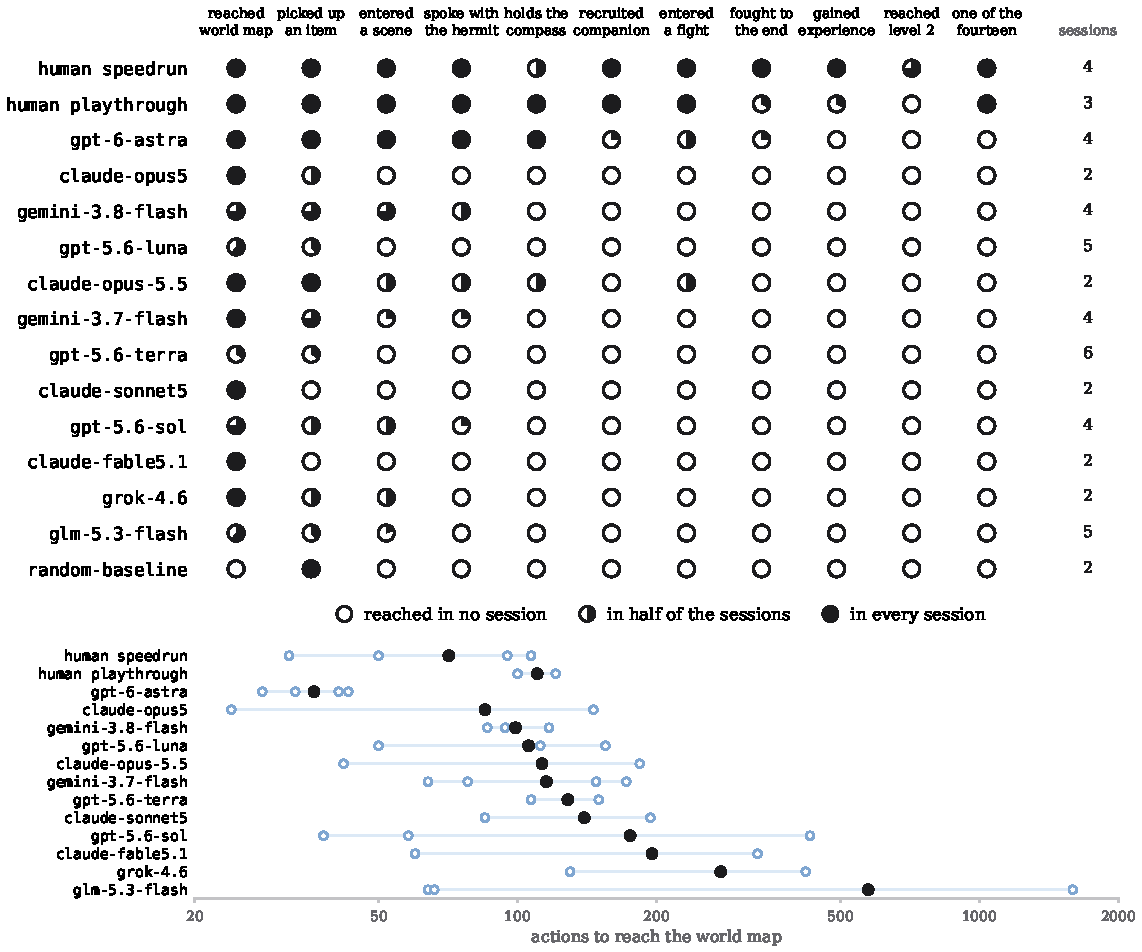
\includegraphics[width=\linewidth]{figures/ladder.pdf}
\caption{Milestones per model, with rows ordered by the mean number of actions to the world map, fewest first, and the random baseline last. In the upper panel each marker shows the share of sessions in which the model reached the milestone, with the number of sessions at the right. The lower panel shows the actions to the world map across the sessions that crossed, on a log scale, with a light dot per session and a black dot for their mean. The two human rows are read from published videos, with a keypress as the action, and \cref{app:measure} gives the record behind each milestone.}
\label{fig:ladder}
\end{figure}

\subsection{Qualitative Analysis}

Four milestones separate the models: the chest, the first scene beyond the home, the hermit and the fight. \Cref{fig:frames} shows one frame from each behaviour pattern behind these divisions. The random policy reaches \QrandomRungs{} of the \Lrungs{} milestones in \QrandomBudgetMin{} minutes, since a random walk in a small room reaches the chest within the hour. No save succeeds during its hour, so the world map is the first milestone a random walk does not reach. The chest therefore separates models from one another but not from the baseline: \Litem{} models searched it and \LnoItem{} never did.

% The frames are fixed evidence from this field, picked by hand from the
% published replays; the labels in the caption are the generated macros, so a
% regenerated field that changes who holds a pattern has to re-pick them.
\begin{figure}[!htb]
\centering
\setlength{\tabcolsep}{2pt}
\begin{tabular}{@{}ccc@{}}
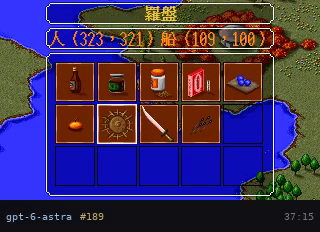
\includegraphics[width=0.32\linewidth]{figures/frames/a-compass-read.png} &
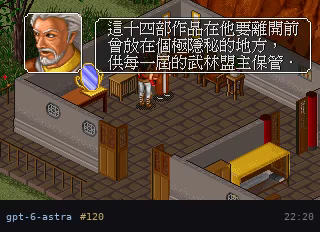
\includegraphics[width=0.32\linewidth]{figures/frames/b-hermit-talk.png} &
\includegraphics[width=0.32\linewidth]{figures/frames/c-recruit-prompt.png} \\
{\footnotesize (a) \LtopLabel} & {\footnotesize (b) \LtopLabel} & {\footnotesize (c) \LtopLabel} \\
\includegraphics[width=0.32\linewidth]{figures/frames/d-first-battle.png} &
\includegraphics[width=0.32\linewidth]{figures/frames/e-cabinet-hint.png} &
\includegraphics[width=0.32\linewidth]{figures/frames/f-fence-corner.png} \\
{\footnotesize (d) \LtopLabel} & {\footnotesize (e) \PtalkSlowLabel} & {\footnotesize (f) \PexitActsMaxLabel} \\
\includegraphics[width=0.32\linewidth]{figures/frames/g-gate-orbit.png} &
\includegraphics[width=0.32\linewidth]{figures/frames/h-inn-loop.png} &
\includegraphics[width=0.32\linewidth]{figures/frames/i-defeat.png} \\
{\footnotesize (g) \PorbitLabel} & {\footnotesize (h) \texttt{grok-4.6}} & {\footnotesize (i) \LtopLabel} \\
\end{tabular}
\caption{Frames from the replays, each with the strip naming the model, the action count and the clock: (a) the compass coordinates on the item screen; (b) the conversation with the hermit; (c) the join prompt of Duan Yu in an inn; (d) a fight; (e) the hermit naming the cabinet; (f) the yard behind the fence; (g) passing the gate of the hermit; (h) talking to an innkeeper; (i) the defeat banner.}
\label{fig:frames}
\end{figure}

Every model crosses onto the world map, in \LcrossSessions{} of the \NsessionsPlayed{} sessions, and \LcrossEvery{} models cross in every session they played. The compound is left through a yard closed by a fence with one gate, and several sessions were stuck in that yard. \PexitActsMaxLabel{} needed \PexitActsMax{} actions to cross in one session and reached the world map at minute \PexitMinMax{} after long stretches of walking into the fence, while the median crossing took \SexitActs{} actions. The count varies more within a model than between models, as the lower panel of \cref{fig:ladder} shows. The crossings of \LspreadLabel{} differ by a factor of \LspreadRatio{} and the means of the models by a factor of \LbetweenRatio{}, while \LtopLabel{} crossed in \LtopCrossMin{} to \LtopCrossMax{} actions in all \LtopSessions{} sessions. Measured by the first save, the \SsaveN{} timed crossings fall between \SsaveFirst{} and \SsaveLast{} minutes into the session, with a median of \SsaveMedian{}.

After the crossing, the rest of the hour is spent on the world map. From it \Lscene{} models entered a scene, for all but \LtopLabel{} an inn or the house of the hermit, and the other \LnoScene{} stayed on the world map or went back into the home. \PorbitLabel{} crossed at minute \PorbitExitMin{}, then spent \PorbitActs{} actions and \PorbitMin{} minutes on the world map without entering a scene, passing the gate of the hermit repeatedly, since the entrance of a walled compound is one tile on one face. \PbatchLabel{} sent lists of up to \PbatchMaxKeys{} keys in one action, \PbatchKeysPerAction{} on average, so it looked at the screen once for every \PbatchKeysPerAction{} keys it pressed.

The second division is the hermit, and it depends on reading his dialogue. \LhermitLabels{} reach his conversation in \PhermitSessions{} sessions, and the conversation is long. \PtalkSlowLabel{} pressed \PtalkSlowPresses{} times through his dialogue at \PtalkSlowPace{} seconds a press, so it took
\PtalkSlowMin{} minutes and ended at minute \PtalkSlowEndMin{}, when the
hermit had named the cabinet and \PtalkSlowLeftMin{} minutes of budget remained. \PtalkFastLabel{} reached him at minute \PtalkFastStartMin{} and pressed \PtalkFastPresses{} times in \PtalkFastMin{} minute. Neither searched the cabinet. \LtopLabel{} reached him in every one of its \LtopSessions{} sessions, between minutes \PhermitTopFirst{} and \PhermitTopLast{}. The \LhermitOthers{} other models that reached him did so in at most \LhermitOthersMax{} of their \LhermitOthersPlayed{} sessions. The compass-holding session that entered the most distinct scenes, \PscenesMax{} within the hour, took \PtalkHolderMin{} minutes over the conversation at \PtalkHolderPace{} seconds a press and searched the cabinet. It then opened the item screen \PholderMenuOpens{} times to read its coordinates from the compass, and all of its \PholderArrows{} arrow-key presses were made inside menus and prompts, none on the world map.

Only one model went beyond the compass. All \LtopSessions{} sessions of \LtopLabel{} read the compass between minutes \PcompassTopFirst{} and
\PcompassTopLast{}, and diverged afterwards. One met Duan Yu
(\game{段譽}) at an inn at minute \PpromptMin{}, answered yes at minute
\PrecruitMin{} when he asked to travel together, and was handed the manual
of his art (\game{六脈神劍譜}). One entered a fight at minute
\PlostFightMin{} and lost it at minute \PdefeatMin{}, then opened the system menu, loaded the save the benchmark had written, and by minute
\PcompassAgainMin{} held the compass again. One entered a fight at minute
\PbattleMin{} and sent its last key at minute \PbattleLastMin{} with the fight still open. The fight is the third and last division, since no model reached a campaign milestone beyond it.

The budget is wall clock, so the compute a model spends on a decision is charged against the time it has left to play, as ARC-AGI-3 and TextQuests charge it \citep{arc2026arcagi3,phan2025textquests}. The clock charges the latency of the provider along with the deliberation of the model, so \cref{app:infra} gives each milestone in actions as well as minutes and lists the pace of every model. The sessions took between \EactsMin{} and \EactsMax{} actions, and the pace did not set the order: the model that reached the most milestones is neither the fastest between actions nor the one that took the most actions in the hour.

\subsection{Four-Hour Sessions}
\label{sec:long}

The \NlongBudgetMin{}-minute budget has \NlongAttempts{} attempts on record. For this archive, a session counts when the service ended it at the budget and either its last key falls within the final \NlongWindowMin{} minutes or reviewed client records show activity continuing until the budget-expiry response, with no observed human interruption. The last key is not the client exit time; an agent that stops sending keys while continuing to inspect the screen is not an interrupted trial. \NlongSessions{} sessions of \NlongModels{} models count, and \cref{tab:long} in \cref{app:infra} gives, for each, the minute of its last key, the minute at which it reached each milestone and its milestone count. The other \NlongWithheld{} attempts do not count: \NlongZero{} sent no action and \NlongStartup{} sent one or two, \NlongEarly{} have neither a last key after minute \NlongMinLastMin{} nor reviewed client-completion evidence, \NlongExcluded{} were declared under names that identify no model of the paper, and one played to the budget with a harness that read the catalogue and the keypress timelines of earlier sessions. That attempt, of \LlongHackLabel{}, held the compass and recruited a companion. While stuck in the opening, the model used its shell to fetch the catalogue and the timelines, ranked them by actions to the world map, and read the key sequences of the fastest, among them a session of \LtopLabel{}. Reward hacking of this kind is common in agent traces \citep{shao2026validity}, and a long horizon gives a stuck model hours to look for it. The sessions that count stay inside the opening: \NlongMap{} of the \NlongSessions{} reach the world map, between minutes \LlongCrossFirst{} and \LlongCrossLast{}, and \NlongScene{} enter a scene. None speaks with the hermit, holds the compass, enters a fight, gains experience or holds a book. The other \NlongPendingModels{} models with four-hour attempts, \LlongPendingLabels{}, have no session that counts.

\section{Conclusion}
\label{sec:conclusion}

We presented \bench{}, a long-horizon benchmark built on a 1996 open-world role-playing game. Every model plays under the same brief and control surface and is scored against events of the game itself. At the \NbudgetMin{}-minute budget, in which a human speedrun finishes the game, the field of \NmodelsDistinct{} models stays inside the opening: every model reaches the world map, \Lhermit{} speak with the hermit, and one, \LtopLabel, takes the compass, recruits a companion and fights, while none gains experience. The stalls fall at the gate of the compound, at the dialogue of the hermit and at the first fight, so the results measure navigation and reading. Combat and the knowledge of the novels, which the campaign tests, remain unmeasured. Four-hour sessions of \NlongModels{} models that play to their budget stay inside the opening. We plan two evaluations. Sessions of eight to twenty-four hours bring the campaign milestones within reach, and a human reference run under the same brief and budget, reported as \citet{wei2025humanbaselines} recommend, calibrates the milestones against a first-time player.

\subsection*{AI use statement}
We used generative AI tools, coding agents built on frontier language models, throughout this work. They implemented the benchmark service, the replay scanner and the scripts that generate every number, figure and table in this paper from the session records. They recovered and reformatted session records, supported the qualitative analysis of the replays, and proposed and refined parts of the measurement design. They searched for and formatted related work, and they drafted and edited the text of this paper under our direction. We have not used generative AI tools to generate synthetic data, to formulate or prove mathematical claims, or to propose hypotheses. The models evaluated in the benchmark are the object of study. We have reviewed all AI-assisted work. Every number in the paper is regenerated from the session records at each build, every typed claim about the records is verified by a consistency script, and the frames and readings behind the qualitative analysis were checked against the replays. We take responsibility for the final content of this work, including text, claims and artifacts produced with the aid of generative AI.

\subsection*{Ethics statement}
The benchmark runs a commercial 1996 game that is not redistributed: every host supplies its own copy, and the frames in this paper identify the interface under study, as \cref{app:licence} explains. The work involves no human participants, and the public catalogue carries the metrics, videos and keypress timelines of model sessions and no personal data.

\subsection*{Reproducibility statement}
The benchmark code, the brief the models receive, the replay scanner and the scripts that generate every number, figure and table in this paper will be released with the paper. The release includes the records, videos and keypress timelines of every session in the field. \Cref{app:infra} lists the emulation and hosting parameters and the dates of the sessions, \cref{app:design} gives the reasons for the protocol choices, and \cref{app:measure} the readings behind every milestone. The game itself is not redistributable, as \cref{app:licence} states.

\bibliography{refs}
\bibliographystyle{iclr2027_conference}

\appendix
\crefalias{section}{appendix}
\crefname{appendix}{Appendix}{Appendices}
\Crefname{appendix}{Appendix}{Appendices}

\section{Release and Licensing}
\label{app:licence}
The benchmark code is released under MIT. The emulation core
(\texttt{dosbox\_pure\_libretro}) is GPLv2 and is loaded at runtime through the libretro C API. The bundled macOS core is built from \texttt{schellingb/dosbox-pure} at \texttt{7f6e8fb}, and the hosted
service ships a Linux build pinned by image digest. The game is the 1996
commercial release, copyright Soft-World International (\game{智冠科技}) and
Heluo Studio. It is not redistributable or tracked in the repository, and every host supplies its own copy. The copy the paper was measured with is identified by two SHA-256 digests. One is of the program file the launcher loads. The other is of a manifest over the 616 shipped files without the three rewritable save slots. The manifest has one line per file, sorted by name, with digest and name.\\ \texttt{\footnotesize Z.DAT\quad 0034f836def2b287e62b0902f08cab22b61b397f24d44d6038274f1750a007ce}\\ \texttt{\footnotesize manifest\quad 29ef75ab32a7905e0b274a9bba9e9ea0ff1b081e74aeacedf86350604aedc558}\\ A copy with another layout yields no reading, as \cref{app:design} explains. The public catalogue therefore carries only the metrics, videos
and replay timelines we measured, and nothing that substitutes for the game
data. The frames of the game in this paper
identify the interface under study, as prior work showing frames of
copyrighted games has done \citep{paglieri2025balrog}. If the rights holders
object, they will be removed.

\section{Interface and Session Details}
\label{app:infra}
\Cref{tab:api} lists the control surface, and \cref{fig:keymap} shows the keyboard the API exposes. A host of 8 vCPUs and 16\,GiB runs up to 24 concurrent sessions. Emulation is DOSBox Pure through libretro at a fixed 26800 cycles, the speed of a 486DX2-66 and period-correct for the game, with no sound card, so the observation is visual only. The published video runs at \DefaultReplaySpeed{} times speed, or faster for long runs, with a strip naming the model, the action number, the keys held and the clock, beside a timeline file with every keypress and its hold. The hour sessions ran from \FieldDates{} and the four-hour sessions from \LongDates{}. Each session is listed under the model that played it, with the thinking level omitted since every session ran at the high level; the name declared to the catalogue differs for \NlongAliased{} four-hour sessions, and the release records the mapping. \Cref{tab:effort} lists the effort of every model in the quantities the service records: sessions, actions, keys per action and the time between actions. The catalogue also holds sessions the paper leaves out: \NexcludedSessions{} of \LexcludedLabel{}, a model with two later versions in the field, and the \NlongWithheld{} four-hour attempts that do not count, each listed in the release with its reason. \Cref{tab:milestones} gives each milestone in actions and in minutes, the medians over the sessions that reached it, read from the replay and its keypress timeline.

Each key is held for a requested number of emulated frames, ten by default, because the game samples its keyboard once per loop. The action returns once the screen has settled: the game has \MsettleReact{} frames to react, and the wait then ends after \MsettleStable{} frames without change, when the picture cycles as in an idle animation, or after \MsettleMax{} frames regardless. A black frame marks a scene change, and the action waits through it and settles once more. A longer animation returns a frame in motion, and the next screen request shows the settled picture. Near the edge of a scene the background stops scrolling and the sprite moves across it, so a model that infers movement from the background miscounts its tiles there, and canopies and roofs can hide the character.

\begin{table}[!htb]
\centering
\caption{The control surface. A check marks a call the model can use in a scored session; the snapshot calls serve development.}
\label{tab:api}
\footnotesize
\begin{tabular}{@{}llc@{}}
\toprule
Call & Meaning & Model can use \\
\midrule
\texttt{GET /api/screen} & the current frame & \checkmark \\
\texttt{GET /api/help} & the brief, in English or Chinese & \checkmark \\
\texttt{GET /api/keys} & every accepted key name & \checkmark \\
\texttt{GET /api/slots} & emulator snapshots on disk & $\times$ \\
\texttt{POST /api/key \{"key":"kp3","hold":10\}} & press one key, or several in order & \checkmark \\
\texttt{POST /api/save \{"name":"..."\}} & take a snapshot & $\times$ \\
\texttt{POST /api/load \{"name":"..."\}} & restore a snapshot & $\times$ \\
\bottomrule
\end{tabular}
\end{table}

\begin{figure}[!htb]
\centering
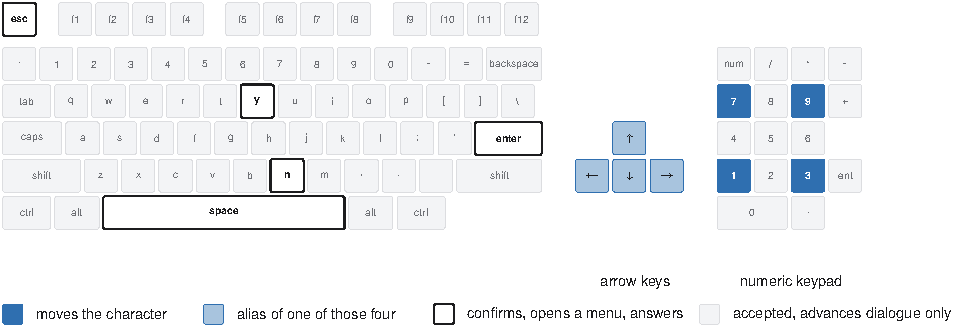
\includegraphics[width=0.8\linewidth]{figures/keymap.pdf}
\caption{The keyboard the API exposes, with the nine keys the game responds to outside dialogue highlighted; any key advances a dialogue.}
\label{fig:keymap}
\end{figure}

\begin{figure}[!htb]
\centering
\setlength{\tabcolsep}{2pt}
\begin{tabular}{@{}cc@{}}
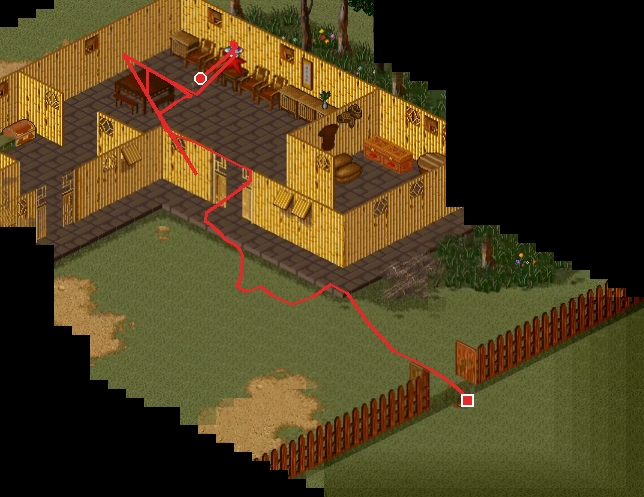
\includegraphics[width=0.41\linewidth]{figures/route-compound.png} &
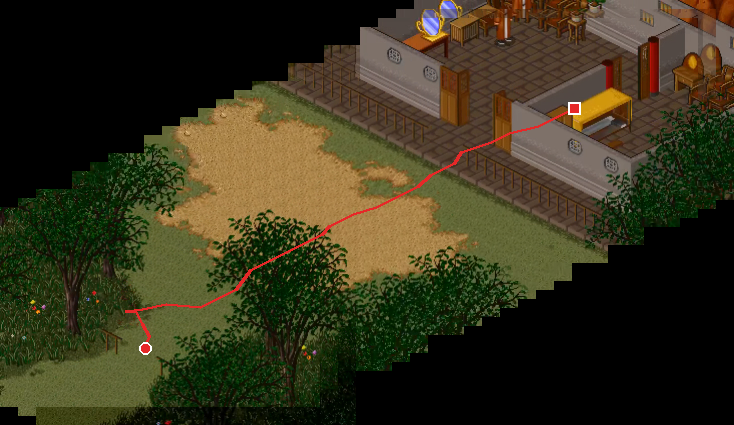
\includegraphics[width=0.55\linewidth]{figures/route-house.png} \\
{\footnotesize (a)} & {\footnotesize (b)} \\
\multicolumn{2}{c}{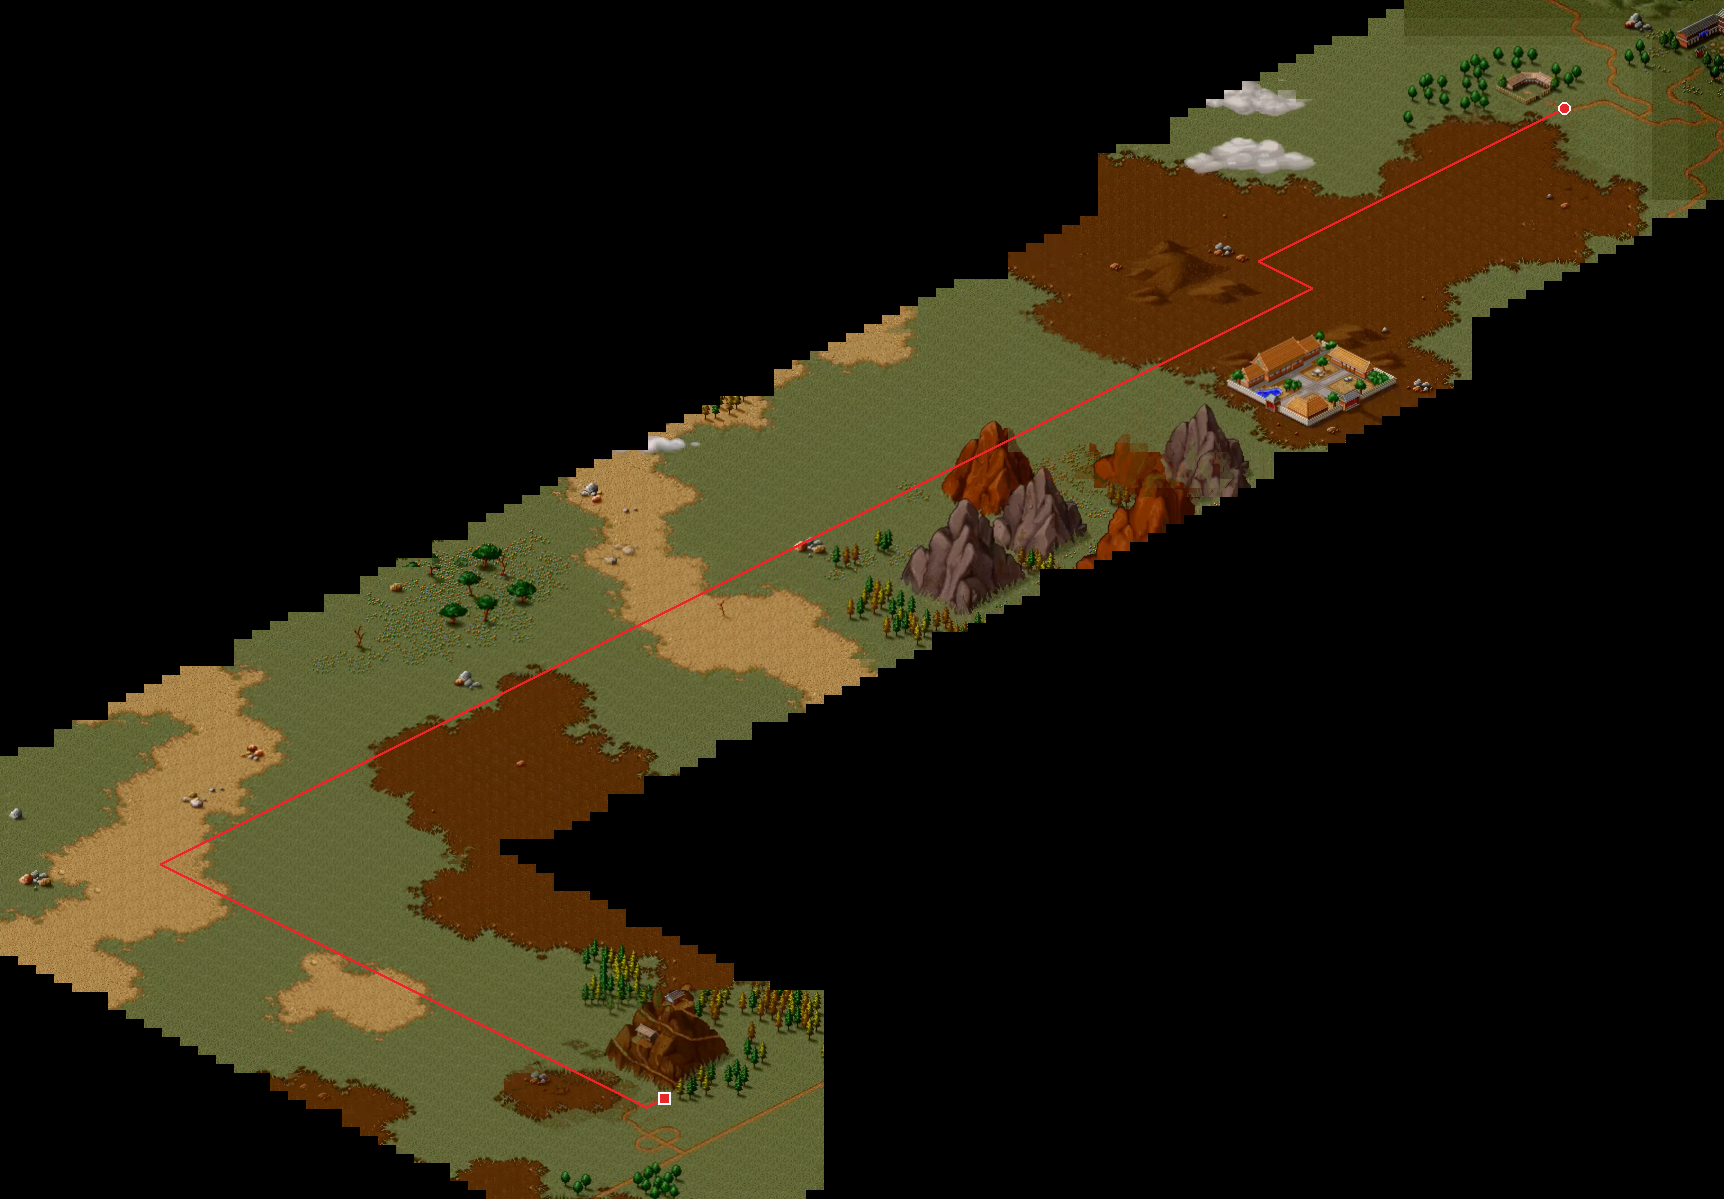
\includegraphics[width=0.93\linewidth]{figures/route-map.png}} \\
\multicolumn{2}{c}{\footnotesize (c)} \\
\end{tabular}
\caption{The opening route as far as the hermit, from a human speedrun: (a) the compound from the spawn tile to the gate, (b) the house of the hermit from its door to the hermit, and (c) the world map between them. In each panel the frames of the walk are registered by phase correlation and merged by a per-pixel median, which removes the hero, and his path is drawn in red from the circle to the square.}
\label{fig:route}
\end{figure}

\begin{table}[!htb]
\centering
\caption{Effort per model in the order of \cref{fig:ladder}; actions and seconds are medians over sessions.}
\label{tab:effort}
\footnotesize
\renewcommand{\arraystretch}{0.86}
% generated by figures/emit_effort.py from the field records; do not hand-edit
\begin{tabular}{@{}lrrrr@{}}
\toprule
Model & Sessions & Actions per session & Keys per action & Seconds between actions \\
\midrule
\texttt{GPT-6 Astra} & 4 & 254 & 3.7 & 11 \\
\texttt{Claude Opus 5} & 2 & 303 & 6.5 & 12 \\
\texttt{Gemini 3.8 Flash} & 4 & 174 & 3.1 & 18 \\
\texttt{GPT-5.6 Luna} & 5 & 155 & 6.9 & 11 \\
\texttt{Gemini 3.7 Flash} & 4 & 170 & 4.9 & 16 \\
\texttt{GPT-5.6 Terra} & 6 & 126 & 11.8 & 12 \\
\texttt{Claude Sonnet 5} & 2 & 369 & 2.8 & 9 \\
\texttt{GPT-5.6 SOL} & 4 & 332 & 3.1 & 8 \\
\texttt{Claude Fable 5.1} & 2 & 874 & 1.4 & 10 \\
\texttt{Grok 4.6} & 2 & 472 & 1.4 & 5 \\
\texttt{GLM-5.3 Flash} & 5 & 215 & 1.8 & 14 \\
\midrule
\texttt{Random Baseline} & 2 & 2118 & 1.0 & 1 \\
\bottomrule
\end{tabular}

\end{table}

\begin{table}[!htb]
\centering
\caption{Each milestone in actions and minutes: the sessions that reached it and the median action count and minute at which they did.}
\label{tab:milestones}
\footnotesize
% generated by figures/emit_milestones.py from the replays and timelines; do not hand-edit
\begin{tabular}{@{}lrrr@{}}
\toprule
Milestone & Sessions & Median actions & Median minute \\
\midrule
reached the world map & 30 & 90 & 18 \\
picked up an item & 20 & 20 & 3 \\
entered a scene & 12 & 145 & 30 \\
spoke with the hermit & 8 & 118 & 27 \\
held the compass & 4 & 130 & 23 \\
recruited a companion & 1 & 269 & 52 \\
entered a fight & 2 & 144 & 33 \\
fought to the end & 1 & 168 & 28 \\
\bottomrule
\end{tabular}

\end{table}

\begin{table}[!htb]
\centering
\caption{The four-hour sessions that count under the rule in \cref{sec:long}: the minute of the last key, the actions sent, the minute at which each milestone was first reached, and the milestones credited. Last key is not client runtime. The crossing is timed by the service and other milestones by the replay; a dash marks a milestone not reached, and no session entered a fight.}
\label{tab:long}
\footnotesize
\setlength{\tabcolsep}{2pt}
% generated by figures/emit_long.py; session IDs are audit comments only
\begin{tabular}{@{}lrrrrrrrrrr@{}}
\toprule
Model & Last key & Actions & Map & Item & Scene & Hermit & Compass & Companion & Battle & Milestones \\
\midrule
% counted-session: ac1e0b048aa4
\texttt{claude-opus-5.5}$^{*}$ & 229.3 & 11850 & 2.9 & 1.2 & 13.2 & 31.2 & 33.6 & -- & 43.2 & 7 \\
% counted-session: bd77396a227d
\texttt{gpt-5.6-sol} & 239.5 & 782 & 19.2 & 210.9 & 90.3 & -- & -- & -- & -- & 3 \\
% counted-session: 8aa37740e5e8
\texttt{deepseek-v4.1-flash} & 239.8 & 6026 & 10.3 & -- & 21.2 & -- & -- & -- & -- & 2 \\
% counted-session: d92f27b88228
\texttt{glm-5.3-flash} & 238.1 & 372 & 48.6 & 3.2 & -- & -- & -- & -- & -- & 2 \\
% counted-session: 7a7f8fa37e88
\texttt{gpt-5.6-luna} & 238.9 & 530 & 9.6 & -- & 125.8 & -- & -- & -- & -- & 2 \\
% counted-session: a5c748b12df1
\texttt{grok-4.6} & 239.4 & 2857 & 14.5 & -- & 148.4 & -- & -- & -- & -- & 2 \\
% counted-session: 2ade73b3f2bb
\texttt{qwen3.8-27b} & 239.0 & 203 & 47.6 & 1.6 & -- & -- & -- & -- & -- & 2 \\
% counted-session: d8bcd235fd6d
\texttt{glm-5.3} & 238.4 & 378 & -- & 45.1 & -- & -- & -- & -- & -- & 1 \\
\bottomrule
\end{tabular}

\end{table}

\section{Design Decisions}
\label{app:design}

An action accepts one key or a list of up to \MmaxKeys{}, because a menu path or a repeated step is one decision. A list costs one round trip and one settle wait for the whole list. The coupling between perception and action is set by how often a model looks, since an action returns no picture unless asked, and a model that sends single keys without asking for the screen is as open-loop as one that sends twenty. The cap bounds the longest list, and every list is recorded in the public timeline.

The observation is the frame the game draws, at its own resolution, since reading sixteen-pixel glyphs and an isometric scene is part of the task and the hermit milestone separates the models on that reading. A text channel or an upscaled frame would score a different task, and a fixed OCR component would put its own errors between the game and every model. Upscaling adds no information, and a model can resample its frame with the tools of its harness. The brief lists the on-screen terms in the Traditional Chinese the game draws. The benchmark scores perception, knowledge and planning together by design, and the milestone order keeps them apart in the analysis.

The scores describe the 1996 release, run as its original binary. A reimplementation such as kys-cpp \citep{scarsty2026kyscpp} has its own timing, text rendering and behaviour, so a track built on it would be a different benchmark. The memory reader confirms the record layout before it reads anything, so a copy with a different layout yields no reading at all.

The baseline is a seeded random policy because it measures what the milestone structure yields to chance: the small first room puts the chest within reach of a random walk, and no later milestone is. A scripted policy would measure the skill of its author, and a trained perception policy would measure its training data, whereas the leaderboard ranks frontier models under one harness. Cradle and Voyager are harnesses, a skill library and a code API around a model \citep{tan2024cradle,wang2023voyager}, so a run through either would rank the harness, and such runs belong on a separate track. The service records keys and frames, so the qualitative analysis reads behaviour from the replay.


\section{Measurement Details}
\label{app:measure}

The world map is read from a save written there or the world-map fingerprint; the item from the bag count or the pickup message; the scene from the name banner drawn on entry, the home excepted; the hermit from his portrait; the compass from the bag or the item screen; the companion from the party size or a yes to the join prompt; the fight from the card of the acting character; the fight fought to its end from the defeat banner or experience gained; experience and level from the character record; and a book from the bag or the player. The archive holds a base block with the world position, the party roster and the shared bag, then \Mrecords{} character records of \MrecordBytes{} bytes and an item table. The memory reader locates the records in the live machine by anchoring on one character name and confirming its two neighbours at the expected stride. A save attempt begins only while no menu is open and after two seconds without a key from the model, and recurs every two minutes and once more before the budget lapses. Inside a scene the escape opens and closes the four-row menu unseen, and in a dialogue it advances one line, at most once in two minutes. A fingerprint of the world map taken from the frame credits the crossing for a session with no save on record.

Every replay frame is matched against the six panels by normalised cross-correlation, and a panel counts when it scores above \ReplayThreshold{} on two consecutive frames. The game holds a panel until a key is pressed, so a single frame above the threshold is a scene transition. The pickup message varies in width with the name of the item, so it is matched along its row, and a single frame counts. A conversation advanced inside one key list shows no panel and is credited from the save, which records the scenes it opened, and a join prompt counts as a recruitment when the first key pressed after it appears is a yes.

The human rows of \cref{fig:ladder} are read from \NhumanVideos{} published videos, \NhumanSpeedruns{} speedruns and \NhumanPlaythroughs{} playthroughs, listed in the release with the frame behind every reading. A capture is admitted when the opening room of a benchmark replay matches it at \HumanRoomGate{} or above, which locates the game frame and excludes the remakes of the game. The capture is scaled to the native frame and matched against the panels as a replay is, over a window of two pixels and at a threshold set per video in the gap of its score distribution. The clock starts where a benchmark session starts, on the first frame in which the hero stands on his spawn tile with his back to the camera, and the crossing is the first black frame after it. An action is a tile step, read from the shift of the background on the lattice of the isometric tile, or a screen change without a step, such as a line of dialogue. A won fight and a level are read from the messages \game{獲得經驗點數} and \game{升級了}, a book from the \game{得到} message that names it, and the ending from the closing conversation with the hermit. A companion is read from the party list, from the manual the first companion hands on joining, or from a fight in which a companion acts.

The readings agree wherever two records exist. The pickup message agrees with the bag on all \PobtainedAgree{} sessions that have both and supplies the item milestone for the \PobtainedRead{} sessions with no bag reading. Of the \SmapBoth{} crossings that carry both a save and a fingerprint, the two agree on \SmapAgree{}, the save credits \SmapSaveOnly{} crossing the fingerprint missed, and the fingerprint never appears without a save behind it. The crossing count read from the replay agrees with the count the service recorded on all \LcrossAgree{} sessions that carry both. Of the \PcompassBoth{} sessions with both a bag reading and a replay, every one of the \PcompassBag{} whose bag holds the compass shows the coordinate line on the replay, and no other session does. Of the \PhermitBoth{} sessions with a preserved save and a replay, every one of the \PhermitOpened{} whose save shows the scenes the hermit opens also shows his portrait on the replay. No frame without a panel scored above \ReplayMissMax{}, and every event has a frame above \ReplayHitMin{}, so any threshold between the two gives the same readings.

\end{document}
